\chapter{Preparation}\label{preparation}

\ifpdf
    \graphicspath{{Chapter2/Figs/Raster/}{Chapter2/Figs/PDF/}{Chapter2/Figs/}}
\else
    \graphicspath{{Chapter2/Figs/Vector/}{Chapter2/Figs/}}
\fi



\section{Balls-into-Bins}


Balls-into-bins models have been studied since the 20th century in probability theory under several different names, e.g.\ ``urn processes'' or ``occupancy problems''~\cite{kolchin1978coined}. A few years later its applicability to real world problems, such as load balancing, has been highlighted, and further research led to the analyses of even more realistic and efficient models. Apart from practical applications, the results derived for balls-into-bins models turned out to be useful in the analysis of several other (randomised) algorithms~\cite{edmonds2006cakecutting}. It is still an actively researched field gaining much attention, and in particular, the main model I will study has been first analysed theoretically in 2019~\cite{dwivedi2019firstthinning} (but known since 1986~\cite{derek1986twothinningfirstattempt}).


\subsection{Assumptions} \label{assumptions}



Load Balancing in the real-world is a very complex task, the optimal solution depends on many specific details and the exact characteristics differ between cases. For example, the servers might (or might not) be different (e.g.\ they serve different types of requests, or they have different speed), the arrival rate of the jobs might be unknown (or maybe an estimated model is possible), servers might crash, etc. Building a theoretical model that is completely general and can still be analysed effectively seems infeasible. Hence, most of the balls-into-bins models capture one or a few characteristics of load balancing, and therefore they are very diverse. Now I present a sufficiently general definition of the balls-into-bins abstraction, and state its assumptions. 

\begin{definition}[Balls-into-bins] \label{definition: balls-into-bins}
In the balls-into-bins problems, there are $n$ bins (servers), and there are $m$ balls (jobs) arriving sequentially. Whenever a ball arrives, it is placed in one of the bins according to a (usually randomised) protocol.
\end{definition}
\NOTE{D}{Maybe add the objective here? Andor: I was thinking about that, but I want to elaborate somewhere on the alternative objective functions.}
\NOTE{D}{A figure would be helpful here. Andor: What kind of figure do you imagine? Do you think this is an important figure to add (space and time constraints etc.)?}

\NOTE{D}{!!This list is quite heavy to read. Maybe you could start by describing the protocols? Andor: why is it heavy to read?}Following are the most important assumptions made by the balls-into-bins model that I will study (and also by the majority of the available literature):


\begin{itemize}
    \item
    Balls never leave the bins. While in most real-world scenarios jobs do end, this model can still provide a good local approximation, or represent the overall work assigned over a time period. Also, most of the theoretical works in the literature analyse the normalised (maximum) load, i.e.\ the difference between the (maximum) load and the average load over all the servers, and this subtraction has a similar type of effect as finishing jobs over time. For other applications, such as hashing~\cite{wieder2017ballsintobinslandscape}, persistent balls are realistic. There are nevertheless some balls-into-bins protocols that include also the deletion of the balls~\cite{azar1999twochoice}, but I will not consider those in this dissertation.
    \item
    The number of balls $m$ is known in advance. As shown in~\cite{feldheim2021longtermthinning}, there are much better strategies for some protocols with this assumption (in terms of normalised maximum load). In many applications, even if $m$ is unknown, it can be estimated from previous runs.
    \item
    The balls and the bins are homogeneous. This assumes that there is just a single type of job (e.g.\ they are of unit size) and all the servers are of the same quality (e.g.\ they have the same speed). These assumptions are valid in several cases, e.g.\ even though Google searches are different, a built-in timeout mechanism makes them approximately unit-sized \NOTE{A}{Reference?}. The more general case of heterogeneous balls and bins has also been analysed, see e.g.~\cite{berenbrink2008weighted}.
    \item
    The randomised protocols are assessed according to the expected value of the maximum load after all $m$ balls have been allocated (\textbf{expected final maximum load}). It is important to emphasize the stochastic nature of the process, that is why we optimise an expected value. Note that while there are several other metrics that can be important for load balancing in practice (e.g.\ expected empirical variance of the final loads, variance of final maximum load, expected maximum normalised load throughout the whole run), only a few papers have considered those so far~\cite{feldheim2021longtermthinning}, so I do not discuss them any further. \NOTE{A}{Should I expand more on what the varience of the load distribution, the variance of the maximum load etc. mean?}
    
\end{itemize}





\subsection{Protocols} \label{protocols}

I will now define the randomised protocols, I will be using in later chapters.


\iffalse % I do not think this paragraph is needed
The general pattern in the protocols below is that they are more robust and are easier to implement than deterministic protocols (as discussed in Chapter~\ref{introduction}), and some of them still provide sufficient guarantees on the objective function (maximum load). The theoretical analysis of the protocols according to the objective function is deferred until Chapter~\ref{evaluation}.
\fi

\paragraph{\OneChoice}

This is the simplest randomised algorithm. The arriving ball is allocated uniformly at random into one of the bins.

\paragraph{\TwoChoice}
\NOTE{T}{I would prefer a more concise, mathematical description of each protocol, clearly separated from motivation etc. Andor: I agree it would be nice, but I am not sure if it is worth the effort to set up some notation, as I do not use it later.}
In this protocol, two bins are chosen uniformly at random (possibly the same two bins), and the ball is placed in the lesser loaded of the two bins . In case of a tie, the ball is allocated uniformly at random into one of the two bins. Implementing \TwoChoice in practice is challenging due to concurrency and communication delays: the servers need to report their loads by interrupting their currently running process; the client has to wait for the response by both servers, and then allocate the job to one of them (one and half round trips).
\iffalse % doesn't add much
A generalisation of \TwoChoice is \KChoice, where not $2$, but $K$ bins are compared.
\fi


\paragraph{\TwoThinning}

This is one of the main protocols I will focus on, and this has been defined in Chapter~\ref{introduction} already.


\iffalse %I should double check, but I think this is all explained in the fst chapter. 
Here I present the main interpretation of this protocol, but in Section\NOTE{T}{Section}~\ref{alternative} I present another way to look at this protocol. An important difference between this protocol, and \KChoice is that this protocol additionally requires a decision strategy, a free parameter of the protocol\NOTE{D}{Maybe remove ``a free parameter of the protocol''}. When a ball arrives, a (primary) bin is chosen uniformly at random, and the according to the strategy, the primary bin is accepted, and the ball is placed into that bin, or it is rejected, and the ball is placed into a (secondary) bin chosen again uniformly at random. \NOTE{D}{This strategy is commonly a threshold function.}The motivation for this interpretation of \TwoThinning is that unlike for \TwoThinning\NOTE{D}{Two-Choice?} where always $2$\NOTE{D}{two} servers are interrupted by a query, here if the primary load is accepted by the strategy, than only $1$\NOTE{D}{one} server is interrupted. A subtlety is that the secondary and primary bins can in fact be the same, while in a real-world application, the client would probably avoid the primary bin if it has been rejected\NOTE{D}{OK, but the improvement is minor}.
\fi

\paragraph{\KThinning}

\KThinning is a generalisation of \TwoThinning. For each ball, up to $k$ bin samples are taken sequentially uniformly at random until one of them is accepted by the decision strategy. In theory, \KThinning provides a major improvement over \TwoThinning~\cite{feldheim2020dthinning, los2021quantilethreshold}.


\paragraph{\GraphicalTwoChoice}
This protocol is a generalisation of \TwoChoice, where only a subset of the pairs of bins can be sampled. Treating the bins as nodes and the pairs that can be sampled as edges of a graph, \GraphicalTwoChoice samples an edge uniformly at random for each ball. It is often assumed that the graph is regular (i.e.\ all nodes have the same degree), otherwise the symmetric final maximum load objective function is not reasonable -- take the star graph as an example of a highly unbalanced graph \NOTE{A}{!! How to cite it properly? Also I feel that this figure doesn't add much, and everyone knows what a star graph is... "Good choice of figures"... I don't remember who suggested me to add this figure.}.

\begin{figure}[hbt!] \label{star-graph}
    \centering
    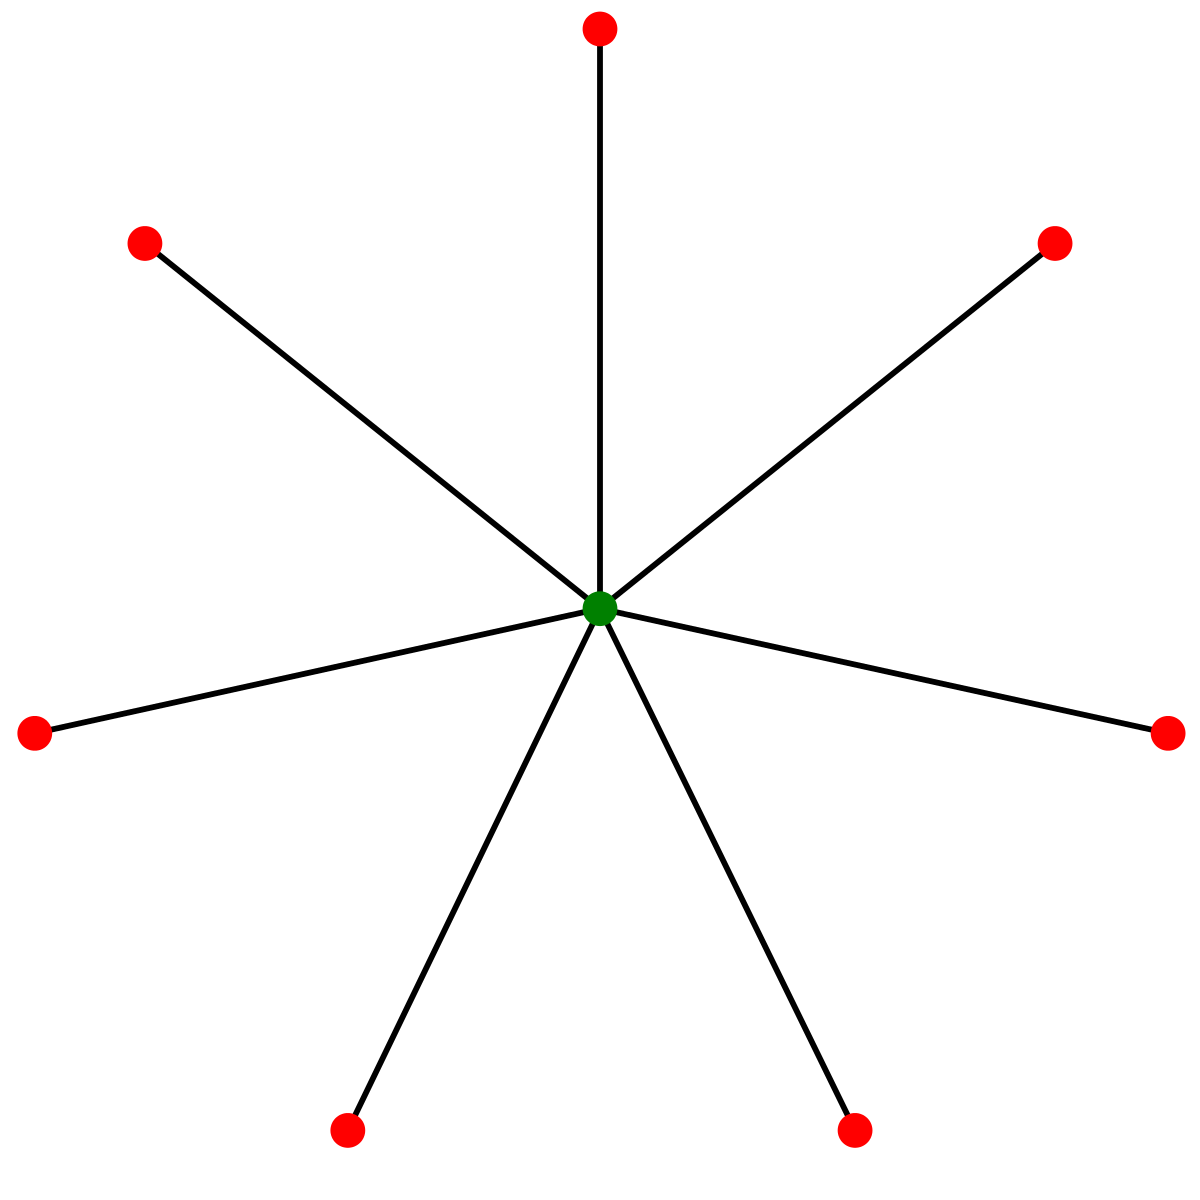
\includegraphics[scale=0.1]{Chapter2/Figs/star_graph.png}
    \caption{Star graph~\cite{stargraph}}
\end{figure}
\NOTE{D}{Maybe it would be good to add a figure of a regular graph or two figures to illustrate how the process works. Andor: agree, it would be nice, but is it worth it? Not sure how much help a figure would be for the reader, or I would have to spend weeks on making that figure.}

The real-world motivation for this protocol stems from the geographical locality of the servers~\cite{krishnaram2006graphicaltwochoiceoriginal}. One possible practical implementation\NOTE{T}{I think this part could be shortened, possibly even removed. Andor: how to shorten it? Do you think it is enough if I had motivation for \TwoThinning and I don't need to motivate \GraphicalTwoChoice?} of \GraphicalTwoChoice for load balancing is that the client chooses a server $A$ uniformly at random, server $A$ queries the current load of a neighbouring server $B$ chosen uniformly at random, and then $A$ decides whether itself or $B$ should complete the job. In this case the edges correspond to nearby servers, but different underlying graphs are also possible~\cite{peres2015oneplusbeta}, and there are other applications as well (e.g.\ for efficient storage of hash tables~\cite{krishnaram2006graphicaltwochoiceoriginal}). For this dissertation, I will make the same simplifying assumptions for \GraphicalTwoChoice as for \TwoThinning. \NOTE{T}{You mean no jobs are removed, and balls are of same size? I think this assumption should be part of the model, and not an addition to the process description. Andor: no... I meant the silly assumption that the full load vector is known. But I feel I shouldn't emphasize it too much as this is the main weakness of the dissertation.}


Note that remarkably, the \Greedy strategy, which allocates the ball into the lesser loaded endpoint of the edge has been shown not to be optimal in general~\cite{bansal2021twochoicegraphical}, and hence this protocol also requires a decision strategy. I present\NOTE{D}{Be sure to mention this in the introduction. It is not guaranteed to be read here. Andor: I agree, it would be nice, but Introduction is already too long. Not sure where I could highlight the important results apart from the Conclusion where I already did. I might think that is enough, but maybe not?} the first known concrete counterexample for the suboptimality of Greedy in Lemma~\ref{lemma: greedy-suboptimal}.


Analogously, \textsc{Graphical Two-Thinning} is a reasonable protocol as well, but I chose to focus on \GraphicalTwoChoice, since there is more literature available on that, and hence a more thorough comparative evaluation is possible.\\


\iffalse
As stated briefly in Chapter~\ref{introduction}, the project is about optimising free parameters of various balls-into-bins protocols. Now with the definitions in hand, we can see that it amounts to finding good strategies for \TwoThinning, \KThinning and \GraphicalTwoChoice. While most of the available strategies are manually defined (e.g.\ choose the lesser loaded, or accept if greater than $x$), I will use algorithms to find good strategies! Hence, I would like to make an important distinction between \textbf{protocol} and \textbf{algorithm}: an algorithm is used to optimise free parameters of a protocol, which can then be used in the balls-into-bins framework with the parameters generated by the algorithm. In particular, I will use RL and dynamic programming as algorithms, to find good strategies for the parametric protocols discussed above. I will use this terminology from now on. On this note, I will use the terms \textbf{decision strategy} and the more general term \textbf{free parameters} interchangeably, always choosing based on the context. \NOTE{A}{Move elsewhere?}\NOTE{D}{Maybe somewhere with the subheading ``notation''}
\fi


\subsection{Definitions and Notation} \label{notation}

For the lemmas and conjectures presented in later chapters, it is useful to define and extend some of the above notions formally as well. Let's denote the integers between $0$ and $n-1$ by $[n]$, indicating the indices of the bins.

\begin{definition}
A \TwoThinning decision strategy is a function $f$, such that for any (sorted) load vector $v$ and bin $i\in[n]$, $f(v, i)\in\{\mathrm{accept},\ \mathrm{reject}\}$.
\end{definition}


\begin{definition} [\TwoThinning decision strategy]
A \TwoThinning decision strategy is a function $f$, such that for any (sorted) load vector $v$ and bin $i\in[n]$, $f(v, i)\in\{\mathrm{accept},\ \mathrm{reject}\}$.
\end{definition}


\begin{definition} [\KThinning decision strategy]
A \KThinning decision strategy is a function $f$, such that for any (sorted) load vector $v$, bin $i\in[n]$ and $0\leq c<k-1$ indicating the number of balls rejected at $v$, $f(v, i, c)\in\{\mathrm{accept},\ \mathrm{reject}\}$.
\end{definition}


\begin{definition} [slicing strategy]
We call a \TwoThinning (or \KThinning in general) decision strategy \textit{slicing}, if it accepts bin $i$ at (sorted) load vector $v$ if and only if its load $v[i]$ is less than or equal to a \textit{threshold} $a$ (that can depend on $v$, and for \KThinning also on the number of bins already rejected for the current ball). \NOTE{T}{The threshold also depends on which stage of $k$-thinning you are? I find the next definition more clearly, and perhaps this one could be dropped? Andor: the problem is the next definition only works for \textit{slicing} \KThinning strategies not any \KThinning strategy, so I need to define what \textit{slicing} means for \KThinning somehwhere... But if I agree with you it would be nice if I could avoid it somehow -- any ideas?}
\end{definition}


\begin{definition} [threshold function]
Note that a \KThinning \textit{slicing} strategy $f$ can be alternatively defined by a corresponding \textit{threshold function} $h^f$, such that $h^f(v,c)$ is the threshold used at load $v$ after $c$  rejected.
\end{definition}



\begin{definition} [monotone strategy]
We call a \KThinning slicing strategy $f$ \textit{monotone}, if $h^f(v,c)\leq h^f(v,c+1)$ for each $v$ and $0\leq c<k-1$. Intuitively, a monotone strategy should never become more selective after rejecting a ball.
\end{definition}


\begin{definition} [expected final maximum load]
Let us denote the expected final maximum load of a (decision) strategy $f$ for a protocol $h$ by $E^f_h$, or $E^f$ when $h$ is implicit from the context.
\end{definition}



\subsection{Notes on Related Work and Background Reading}

\NOTE{A}{Give more concrete examples?!}
\NOTE{D}{I think you have already demonstrated that you have read the prior work by the numerous references that you have. Andor: So should I cut down on this section?}
\NOTE{D}{I think a clear way to demonstrate that you have researched the prior work, would be to create a table with the processes and theoretical gap they achieve in the lightly loaded and heavily loaded case. (you can find something like this in prior work). Andor: I disagree, as those gaps are not directly useful for my project, and this section points out some nice insights on the other hand. But you can convince me.}

As part of the preparation I was reading several papers about the theory of balls-into-bins. Now I present my main findings: 


\begin{itemize}
    \item 
    I wanted to understand why there are so many different protocols, see how they are interconnected, and explore the main directions of current research. These allowed me to choose in a principled way which protocols to focus on. In particular, \TwoThinning, the main protocol of my study, has been analysed as a resource efficient protocol in-between \OneChoice and \TwoChoice. (We can see a similar phenomenon with the so-called \textsc{($1+\beta$)-process}~\cite{peres2015oneplusbeta}).
    \item
    I found that most of the papers in this area approach the topic from a theoretical viewpoint, and there is a big gap between these results and the practical applications. Even though my approach is also a theoretical one, I found it important to gain practical motivation, and therefore I actively searched for papers bridging this gap (e.g.~\cite{wang2017twochoicerouting}).
    \item
    As preparation for formulating my own lemmas and conjectures for the dissertation, I wanted to gain an insight into how lower and upper bounds can be derived theoretically on the maximum load of various protocols. Therefore I studied several proofs, e.g.\ that \TwoChoice achieves a maximum load of $\frac{\ln(\ln(n))}{\ln(2)} + O(1)$ after $n$ balls~\cite{azar1999twochoice}. These proofs did not just provide insights into why or why not different protocols work well, but the proofs also provide intuition for improving protocols, or what is even more important for my project, creating good strategies. For example, the so-called \Threshold strategy for \TwoThinning is based on the observation that rejected balls form a \OneChoice process, for which tight bounds are available~\cite{feldheim2021thinning}.
    \item
    Perhaps surprisingly, the more general case where $m\geq n$ is much more challenging than the $m=n$ case (i.e.\ where the number of balls equal the number of bins)~\cite{berenbrink2006heavilyloaded}. In real-world applications this assumption may usually not hold, only if the number of jobs is somehow controlled. As we will see in Chapter~\ref{implementation}, my approaches will not be limited by this constraint.
    \iffalse % I discussed it all already in the Introduction, I think
    \item
    Almost exclusively all of the proofs are asymptotic -- they only hold for very large $n$, mostly due to approximations, such as Stirling's formula~\cite{feldheim2021thinning}. This is very restrictive for real-world applications, as discussed in Chapter~\ref{introduction}. Similarly, (and sometimes also as a consequence of the above), the bounds hold only up to a constant/logarithmic factor, i.e.\ they are fixed only up to the $\Theta$ notation. In particular, there exist strategies that have been shown to be optimal for \TwoThinning, such as the ``$\ell$-threshold strategy'' for $m=n$, but this is also not necessarily optimal for practically realistic values of $n$ and $m$! \NOTE{A}{Better phrasing. An interesting idea that I will get back to in Chapter~\ref{evaluation} is trying to find out or bound the constant factors hidden behind the $\Theta$ notation, which would be very useful for comparisons.}
    \NOTE{D}{This sounds interesting}
    \fi
\end{itemize}

\NOTE{D}{This should also be in the introduction and conclusions. Andor: would be nice, but there are no words remaining for that :(}
Combining many of the above points, to the best of my knowledge my work is novel in several aspects. The decision strategies I find using algorithms such as dynamic programming (DP), are optimised for a specific value of $n$ and $m$, and hence have the capacity to outperform the asymptotically optimal, manually defined strategies. In particular, using dynamic programming, I find the optimal strategies for moderate values of $n$ and $m$, exploiting that the state space is finite (i.e.\ there are just finitely many load configurations), which is the first such analysis to the best of our knowledge.


\section{Reinforcement Learning} \label{RLintro}


In the Part IB Artificial Intelligence course we have been introduced to supervised learning. While Reinforcement learning (RL) is also about optimising an objective function, it differs in several aspects (e.g.\ no labelled data, interactive environment). A very readable introduction to RL can be found in~\cite{sutton2018RLbook}, expanding on my explanation below.


In RL, there is an agent that is trying to learn an optimal policy by interacting with an environment. It starts in a start state\NOTE{T}{odd formulation. Isn't the point that the start states has no training set/no initial information? Andor: can you explain a bit more? Doesn't the next sentence make this one clear?}, carries out an action, receives a reward from the environment, observes a new state, and repeats this process until it reaches an end state. This process (game) is executed (played) several times (one such run is often called an ``episode'' or ``epoch''), until a sufficiently good policy is learnt. There are several versions of RL, e.g.\ depending on what we are optimising exactly, but there is a common underlying mathematical model, the so-called Markov Decision Process that I will introduce next.\NOTE{T}{Make this more precise. I do not think MDP cover everything in RL learning. Andor: are you sure? I would think it does cover most of it, and certainly what we need. Can you give some concrete examples of what are missing?}

\subsection{Finite Markov Decision Process (MDP)}


The main component of a Finite MDP is the environment consisting of the following:
\begin{itemize}[itemsep=0pt]
    \item $S$: state space
    \item $s_0$: start state
    \item $S_f$: set of final states
    \item $A(s)$: action space available at state $s$
    \item $R(s, a, s')$: possible rewards after executing action $a$ in state $s$ and observing next state $s'$
    \item $P(s', r \mid s, a)$: the probability of receiving reward $r$ and transitioning to state $s'$ after executing action $a$ in state $s$
\end{itemize} 


The Markov property has to hold: the transition and reward probabilities are independent of the past, and depend only on the current state and the action executed. Using timesteps as indices \NOTE{A}{Is this clear?}, it means\NOTE{D}{You could replace this sentence with ``More formally,''. Andor: but then I don't define what $_{t}$ means, is it not a problem?}
\begin{equation} \label{eq:MarkovProperty}
P(s_{t+1},r_{t} \mid s_{t}, a_{t}, s_{t-1}, a_{t-1}, s_{t-2}, a_{t-2}, ..., s_{0}, a_{0}) = P(s_{t+1},r_{t} \mid s_{t}, a_{t})\text{ .}
\end{equation}


The other component of the MDP is an agent that has to learn a policy,\NOTE{D}{The agent has to learn a \textit{policy}, ..} i.e.\ a function $\pi(a\mid s)$ that assigns probabilities to each of the executable actions in any state. The goal of the agent is to maximise the expected (discounted) cumulative reward collected\NOTE{D}{until the end state:} during an execution of the game:
\begin{equation}\label{eq:cumReward}
\mathbb{E}_{\pi}[r_{0} + \gamma r_{1} + \gamma^2 r_{2} + \gamma^2 r_{3} + \ldots]\text{ ,}
\end{equation}

where $\gamma \in [0, 1]$ is the discount factor, and the sum goes until an end state is reached. Discounting is needed mainly for possibly infinite, or unbounded MDPs (i.e.\ where a game can last arbitrarily long) to avoid divergent rewards. As we will see in Chapter~\ref{implementation}, all our MDPs are finite and bounded -- often even have a constant number of steps -- so I will set $\gamma=1$ and I will not discuss the more general case from now on. \NOTE{A}{Maybe say that reward shaping has a comparable effect to discounting anyways.}


During ``training'', the agent leans the policy by playing the game several times, i.e.\ starting from the start state, and then interacting with the environment using an arbitrary policy, until an end state is reached.\\

An example MDP is (a simplified version of) what I will use for \TwoThinning:

\begin{itemize}[itemsep=0pt]
    \item 
    $S$: load vectors $\{v\in \mathbb{N}^n\mid\mathrm{sum}(v)\triangleq \sum_{i=0}^{n-1}v[i]\leq m\}$
    \item
    $s_0$: the load configuration no balls
    \item
    $S_f$: load configurations with $m$ balls
    \item
    $A(s)$: integer thresholds $0\leq a\leq m$ (meaning that bins with load at most $a$ are the ones accepted)
    \item
    $R(s, a, s')$: the reward is $0$ for $\mathrm{sum}(s')<m$ and $-\mathrm{maxload}(s')\triangleq -\max_{i=0}^{n-1} s[i]$ for $\mathrm{sum}(s')=m$
    \iffalse
    a primary bin is sampled, and if it is rejected according to $a$, then a secondary bin is chosen. Allocating the ball into the primary or secondary bin, we get $s'$, the new load configuration. If $s'$ has all the $m$ balls, then the reward is $-maxloadvalue(s)$, otherwise there is no reward, i.e.\ it is $0$.
    \fi
    \item
    $P(s', r \mid s, a)$: the probabilities are derived according to the rules of \TwoThinning
\end{itemize}
\NOTE{D}{Add commas to the bullet points (and full-stops) in the last one}


\subsection{Fundamentals}

Now I define some notions that will be useful for the RL and DP algorithms.\NOTE{D}{Maybe name this section DP? Andor: it is a good idea to give it some name as it is not really about the MDP. Even though I agree and understand what you mean by DP, I think it might be a bit misleading for the reader? So I chose ``Fundamentals'', let me know your thoughts.}


We define the \textit{state-value function}, the expected cumulative reward of a policy starting from state $s$ as:

\begin{equation}\label{eq:statevalueFunction}
V_{\pi}(s)=\mathbb{E}_\pi[G_t \mid s_t = s] \text{ ,}
\end{equation}

where the random variable $G_t$ is defined as $r_{t} +  r_{t+1} + r_{t+2} + \ldots$.

When $s=s_0$, we get the expected total cumulative reward of a policy $\pi$, exactly what we aim to maximise. Hence, the optimal policy $\pi^*$ is defined by $\pi^* = \argmax_{\pi} V_{\pi}(s_0)$.


Similarly we define the \textit{action-value function}, the expected cumulative reward of a policy starting from state $s$, choosing action $a$ as:

\begin{equation}\label{eq:actionvalueFunction}
Q_{\pi}(s, a)=\mathbb{E}_\pi[G_t \mid s_t = s, a_t = a] \text{ .}
\end{equation}


The basis of most of the learning algorithms are the Bellman equations~\cite{bellman1957bellmanequation}, that characterize the optimal policy:


\begin{equation}\label{eq:bellmanState}
V_{\pi^*}(s) = \max_a \mathbb{E} [r_t + V_{\pi^*}(s_{t+1}) \mid s_t=s, a_t=a]
\end{equation}


\begin{equation} \label{eq:bellmanAction}
Q_{\pi^*}(s,a) = \mathbb{E} [r_t + \max_{a'} Q_{\pi^*}(s_{t+1},a') \mid s_t=s, a_t=a ] 
\end{equation}
\NOTE{T}{use equation* instead of equation, if you do not cite these equations! Andor: I didn't know about this rule, thanks for letting me know. To my eyes it feels strange to have some numbered and unnumbered equations mixed.}

\iffalse % Maybe this can be dropped, this just confuses the reader, and I explain most of it for Policy Gradient.
Note that there is always a deterministic optimal policy. On the other hand, some learning algorithms use randomised policies as intermediate policies during training, mainly due to technical reasons. Also, an important property that will hold in most of my protocols is that the model of the environment is known to the agent -- otherwise, a deterministic policy might not be optimal, due to state aliasing \NOTE{A}{I am not sure how to add references to these, which are all explained in the book, and these are kind of basic facts.}.
\fi

Even with these equations, finding the optimal policy is not trivial. The two main difficulties are 1) the possible cycles while moving around the state space and 2) the exponentially large size of the state space. As we will see in Chapter~\ref{implementation}, in our case the state transition graph is acyclic, so the former is not a problem. However, in general, to deal with the latter, the optimal policy has to be approximated.



\subsection{Algorithms}


In all of our protocols the state space is large (the number of ways $m$ balls can be placed in $n$ bins is exponentially large), so the agent can focus only on a subset of the states and actions during training. It has to balance between exploring new actions (possibly leading to new states), and gaining confidence in its top actions. This is more generally known as the exploration-exploitation trade-off~\cite{kaelbling1996explorationexploitation}.

The most common approach for dealing with the exploitation-exploration trade-off is the $\epsilon$-greedy technique. During training, the currently best action is chosen with probability $1-\epsilon$ (exploitation) and otherwise the action is chosen uniformly at random (exploration). After training, we set $\epsilon=0$.



\subsubsection{Q-Learning}


Q-Learning~\cite{watkins1989qlearning} uses the action-value function based Bellman equation~\eqref{eq:bellmanAction}. The algorithm maintains a so-called ``Q-table'' $Q(s,a)$, which stores the current estimates of action-value function $Q_{\pi^*}(s,a)$ of the optimal policy. The agent plays the game several times using the $\epsilon$-greedy technique to choose the next action in state $s$ based on the Q-table at state $s$. After every step, it updates the Q-table using a linear interpolation with smoothing factor $\alpha \in (0,1)$ according to the following update rule:

\begin{equation} \label{eq:q-learningUpdate}
Q(s_t,a_t) \leftarrow Q(s_t,a_t) + \alpha\left( r_t + \max_{a'} Q(s_{t+1}, a')) - Q(s_t,a_t)\right) \text{ .}
\end{equation}
\NOTE{D}{Did you see comment about changing $Q$ to $\hat{Q}$? Andor: I think it is standard notation to use simply $Q$, but I see your point. I think it is reasonable to leave it as it is unless you have very strong objections.}


\subsubsection{\DQL} \label{deepq-learning}


Q-Learning, and its iterative approximation method is a good choice for moderately sized state spaces, where more direct (mainly dynamic programming) methods are infeasible. However, for exponentially large state spaces (as in our case), it is infeasible to store the Q-table. In \DQL~\cite{mnih2013DQN}\NOTE{A}{Is $\sim$ needed? How does it work with xspace?}, the Q-table is approximated using a neural network $Q_w$ with a tractable number of weights $w$.

Since with function approximations it is not possible to update $Q_w(s, a)$ in isolation, the update rule also has to be adjusted. A natural choice would be to use the gradient of the squared error between the old and the new estimate:

$$\frac{\partial (( r_t + \max_{a'} Q_w(s_{t+1}, a')) - Q_w(s_t,a_t))^2}{\partial w} \text{ .}$$

In practice, due to stability reasons~\cite{barnard1993semigradient}, \NOTE{A}{Check that I am not saying something stupid.} a semi-gradient is used instead, which essentially treats $Q_{\mathbf{w_t}}(s_{t+1}, a')$ independent of $w$ for the purpose of the differentiation. This yields the final update rule:


\begin{equation} \label{eq:deep-q-learning-update-with-semi-gradient}
\mathbf{w} \leftarrow \mathbf{w} + \alpha\left( r_{t+1}+ \max_{a'} Q_{\mathbf{w}}(s_{t+1}, a') - Q_{\mathbf{w}}(s_t,a_t)\right)\nabla Q_{\mathbf{w}}(s_{t}, a_t) \text{ .}
\end{equation}

Following standard terminology, I will call the NN used by \DQL as a Deep Q-Network (DQN).

\subsubsection{Alternatives}

There are several other algorithms and variants, some of which I implemented and did not outperform \DQL -- see Appendix~\ref{alternativeRL} for further discussion.


\subsection{Recurrent Neural Networks} \label{RNN}


I experimented with several NN architectures for $Q_w$, and here I introduce those that were not covered in the IB Artificial Intelligence or other courses.

Recurrent neural networks (RNN)~\cite{hopfield1982RNNoriginal} process sequential information, by using a hidden state, and updating it by a common weight matrix on every new input (see Figure~\ref{RNN-image}). I will use RNNs to obtain an embedding of the load vector (and not to produce an output sequence).

\begin{figure}[h]
    \centering
    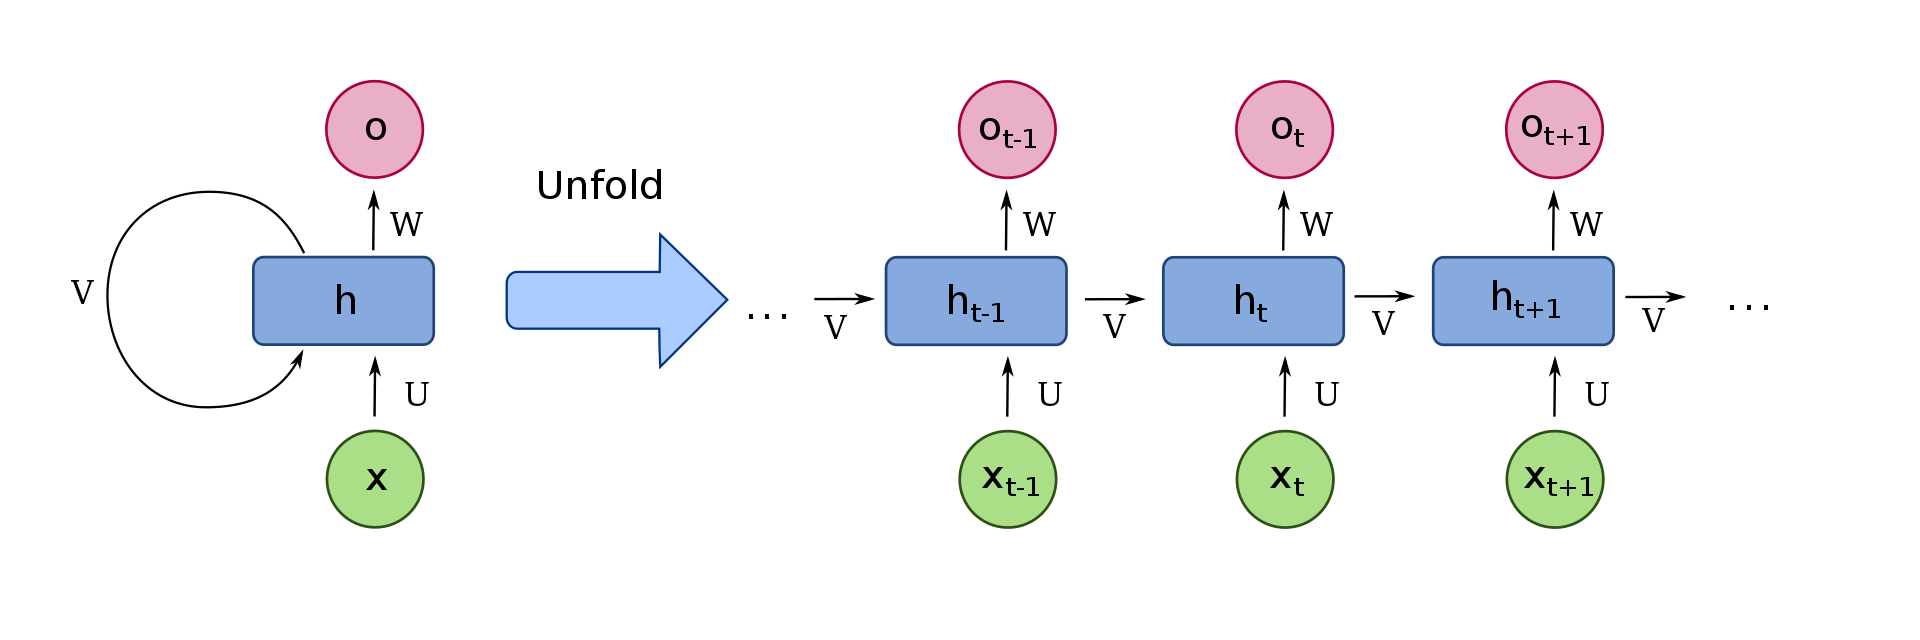
\includegraphics[scale=0.2]{Chapter2/Figs/RNN.png}
    \caption{Two ways of thinking about RNNs~\cite{RNN}.}
     \label{RNN-image}
\end{figure}

There are more complex versions of the vanilla RNN\NOTE{D}{Make sure that it is clear this is the RNN in Elmer. Andor: I don't understand this sentence.} that can remember earlier inputs more (and be less susceptible to the vanishing/exploding gradient problem~\cite{noh2021rnnvanishinggradient}) by using some kind of gating mechanism controlling how much the hidden state is overwritten. The two most notable such architectures are GRU and LSTM (see~\cite{shewalkar2019rnngrulstm} for a thorough comparison).

% \section{Real World and Balls-into-Bins} \label{alternative} I think I explained enough motivation all throughout, no need for more.

\iffalse
There are several ways to make the abstract balls-into-bins model more realistic. Let's\NOTE{T}{Let us} take \TwoThinning as the running example. One idea is not to keep track of the full load distribution, but instead store just some summary. This would require less amount of shared state on the servers, and make the protocol possibly more distributed. On the extreme, using no shared state at all, all clients could use a global threshold when accepting/rejecting primary servers, making it a completely distributed protocol. Something in-between could be storing the overall load of the system, that is the number of jobs present overall on the servers. I will discuss the implementation for these ideas in Section~\ref{lesssharedstate}.


As I mentioned in Section~\ref{protocols}, there is an alternative interpretation of most of the protocols, and in particular, \TwoThinning, that goes as follows. A client chooses a server uniformly at random, since it doesn't have any knowledge about the load values of the servers. The chosen server (not the client!) has access to the load values of all the servers, and based on that information, it decides if it takes the job itself, or concludes that it is overwhelmed, in which case it gives the jobs to another server chosen uniformly at random. After the job is allocated, the servers synchronise their information about the new load values. Theoretically, this is the same \TwoThinning protocol, but here the client doesn't query a load, instead, the primary server makes the decision itself.


We still have to address the question of why to choose the secondary server at random if the primary server cannot take the job. Why doesn't it give the job to the least loaded server? To answer this question we have to look at the so-called Batched protocol. In this protocol, the servers synchronise their load values only in every $T$ steps, or more realistically after every $t$ seconds. This means that they are using outdated load information when choosing which server to give the job. This might lead to each server choosing the previously least loaded one, and seriously overloading it until the new information gets synchronised. To prevent this, a reasonable strategy is to choose the secondary server uniformly at random, leading to the final alternative interpretation of \TwoThinning. In this dissertation I do not consider this practical path any further, I just found it important to give practical evidence as well to the theoretical work.
\fi


\section{Starting Point}

The starting point is exactly as stated in my project proposal ( see Appendix~\ref{proposal}). \NOTE{A}{!!Should I add anything else? I really do not know what they want here.}


\section{Software Engineering Methodology}


\NOTE{A}{Maybe add something about how the goal of the project has been shaped during the year?}



\subsection{Software and Hardware}


For this project I used Python, due to 1) its flexibility for quick experimentation, 2) extensive library support with strong community (e.g.\ numpy~\cite{harris2020numpy} for vectorised computation, Pytorch~\cite{paszke2019pytorch} for deep learning) and 3) its object oriented features. I used the PyCharm IDE for its powerful debugger and its ability to seamlessly parallelise tasks.


I used my laptop for all experiments -- its details are: \texttt{Intel(R) Core(TM) i7-8565U CPU @ 1.80GHz, 1992 Mhz, 4 Cores, 8 Logical Processors, NVIDIA GeForce MX150 GPU}\NOTE{A}{Is this texttt style really better, Dimitris? It looks ugly.}. Gaining the expected speedup from GPUs for RL is not an easy problem, due to the difficulty of batching for a MDP~\cite{stooke2018gpudeepRL} (see Section~\ref{evaluationnotes} for my approach).


\subsection{Project Management}

I used Git for version control and Google Drive as a secondary backup, taking monthly copies. I used the work plan in my project proposal as the target schedule, interleaving evaluation and implementation work to gain better insights about what to focus on. I also maintained a logbook that later served as the baseline for my dissertation. We had biweekly meetings with my supervisors, where we came up with several ideas\NOTE{D}{Maybe the rest of the sentence can be dropped? Andor: hm maybe, but otherwise the sentence says nothing} and analysed my results from the perspective of the closely related research they are doing. I used \LaTeX for writing this dissertation.

\iffalse
I used Git for version control -- it served as my primary backup, and also provides an easy-to-follow progression of my project via the commits. I additionally used Google Drive as a secondary backup, taking monthly copies. \NOTE{D}{Does this belong to the previous section? Andor: No.}

I used the work plan in my project proposal as the target schedule, and while my project has been on track throughout the whole year, it turned out to be beneficial to interleave evaluation and implementation work packages to gain better insights into what parts of the implementation to improve on. I also maintained a logbook, noting down all the todos and a summary of the work that has been completed. This logbook served as the baseline for my dissertation.

We had biweekly, and sometimes weekly meetings with my supervisors where we carefully assessed the progress of the project, and brainstormed several possible ideas for improvement and extension -- some of which I did not have time to implement\NOTE{D}{fully explore} and I mention in Chapter~\ref{conclusion}.

I used LaTex for the dissertation, due to its support for custom formatting, references, and mathematical notation. I have written the dissertation in Overleaf, an online LaTex editor, due to its collaborative features, that made it easy to exchange comments with my supervisors. I also included the dissertation in the Git repository, regularly updating from Overleaf.

\NOTE{A}{Maybe risk saying some fancy Spiral methodology?}
\fi

\subsection{Requirements Analysis and Risk Assessment}

Now I present the risk assessment of the requirements of the project, which helped me prioritise components.

\begin{itemize}

    \item \textbf{Background Reading}: \textcolor{YellowOrange}{medium risk}, \textcolor{Red}{high difficulty}
    
    I had no previous knowledge about RL or balls-into-bins, beyond related foundational courses from the Tripos, so I have done extensive background reading in both, gaining a deep understanding of the balls-into-bins literature, and explored the relevant parts of RL.
    
    The biggest challenge was understanding the proofs in balls-into-bins papers, which I considered an extension. I eventually succeeded and gained valuable insights.
    
    \item \textbf{Implementing Deep Reinforcement Learning}: \textcolor{red}{high risk}, \textcolor{red}{high difficulty}
    
    The main risk involved in this main component was the uncertainty whether RL, being a novel approach to balls-into-bins, will actually perform well in optimising decision strategies. \iffalse However, I want to emphasize that the goal of the project was to investigate how applicable it is, not showing that it is applicable. Eventually, RL was successfully applied, but some questions remain about its usefulness, as discussed in Chapter~\ref{conclusion}. \fi
    
    The main difficulty was optimising \DQL for better results (see Section~\ref{improvementideas}).
    
    \item \textbf{Implementing Other Strategies}: \textcolor{green}{low risk}, \textcolor{YellowOrange}{medium difficulty}
    Having done much competitive programming, I was confident in my algorithmic knowledge, so I could efficiently develop and implement algorithms, such as dynamic programming.
    
    \item \textbf{Evaluation}: \textcolor{YellowOrange}{medium risk}, \textcolor{YellowOrange}{medium difficulty}
    
    The medium risk stemmed from the novelty of my non-asymptomatic approach, and the time it took to compare the strategies with acceptable confidence intervals.
    
    The hardest part about evaluation was finding the most insightful analyses for explaining the behaviour of strategies.
    
\end{itemize}